\section{System Model}
\label{sec:model}
% In this section, we elaborate the model of edge computing systems with random job arrivals, uploading latency and computation time,
% as well as the signaling mechanism with periodic broadcast.
%----------------------------------------------------------------------------------------%

\subsection{Network Model}
We consider an edge computing system with $K$ Access Points (APs), $M$ edge servers, and $1$ cloud server as illustrated in Fig.\ref{fig:system}.
The set of APs and processing servers are denoted as $\apSet \define \set{1,\dots,K}$ and $\esSet \define \set{0,\dots,M}$, respectively.
Specifically, we have \comments{\emph{processing server} denote both edge servers and the cloud server for job processing} and the $0$-th processing server denote the cloud server.
\comments{One edge server is always collocated with one AP, i.e., the edge server is deployed at the same place with the access point.}
Each AP collects the jobs from the mobile users within its coverage, and makes dispatching action on the processing servers for each job.
Furthermore, it is assumed that one AP could only access to the cloud server, the collocated edge server if existed, and neighbor edge servers \comments{(i.e., the pair of edge servers connected via the routing path as illustrated in Fig.\ref{fig:system})} due to transmission latency limitation.
% It is assumed that the $k$-th AP only dispatches the computation jobs to the edge servers within a certain number of hops.
% Let $\esSet_{k} \subseteq \esSet$ be the subset of edge servers which can compute the jobs from the $k$-th AP, and $\apSet_{m}$ be the subset of APs, which may upload jobs to the $m$-th edge server.
We refer to $\esSet_{k} \subseteq \esSet$ as the \emph{candidate server set} of the $k$-th AP,  $\apSet_{m} \subseteq \apSet$ as the \emph{potential AP set} of the $m$-th edge server, and $\rho_{k,m}$ as the collocation indicator (i.e., $\rho_{k,m}=1$ if $k$-th AP and $m$-th edge server collocated, otherwise $\rho_{k,m}=0$) ($\forall k\in\apSet, m\in\esSet$).
% Different APs may have different candidate servers according to their locations in the network, as illustrated in Fig.\ref{fig:system}.
We consider cloud server as one special processing server with stronger computation capability, but also with larger transmission latency compared with the edge servers.
% In this edge computing network, each AP and edge server periodically broadcast their state information (the state information is defined in the Section \ref{subsec:broadcast}), and one AP updates its strategy of job dispatching when receiving the broadcast state information.

%NOTE: [job space support and arrival process]
The dispatchers are implemented on the APs in a distributed manner.
% which would suffer from heavy communication overhead with other AP nodes but with powerful computation capacity.
% In this paper, we shall optimize the job dispatching strategy distributed at APs with partially observable state information, where both job uploading and state information broadcasting suffer from random transmission latency.
Without loss of generality, it is assumed that there are $J$ types of jobs computed in this system, which are denoted via the set $\jSpace \define \set{1,\dots,J}$.
The time axis of job dispatching is organized by time slots.
The arrivals of the type-$j$ jobs at the $k$-th AP ($\forall k\in\apSet,j\in\jSpace$) in different time slots are assumed to be independent and identically distributed (i.i.d.) Bernoulli random variables, and the arrival probability is denoted as $\lambda_{k,j}$.
% Let $B_{k,j}(t) \in \set{0,1}$ represent the event of job arrival, where $B_{k,j}(t)=1$ means one type-$j$ job arrives at the $k$-th AP in the $t$-th time slot, and $B_{k,j}(t)=0$ means otherwise.
% Hence,
% \begin{align}
%     \Pr\{ B_{k,j}(t) = 1 \} = \lambda_{k,j}, \forall t,k\in\apSet,j\in\jSpace.
% \end{align}
%NOTE: [uploading process]
Each AP immediately dispatches each type of arrived jobs to one processing server.
\comments{It's assumed that the network traffic over the routing path is random, and the job uploading from one AP to one edge server consumes a random number of time slots.}%
%Due to the random traffic in the network, the job uploading from one AP to one edge server consumes a random number of time slots.
% It is assumed that the random uploading latency are independent for each job.
Let $\mathbb{U}_{k,m,j}(\Xi)$ be the uploading latency distribution of the type-$j$ jobs from the $k$-th AP to the $m$-th server with finite support $\set{1, \dots, \Xi}$ ($\forall k\in\apSet, m\in\esSet, j\in\jSpace$), whose expectation is denoted as $u_{k,m,j}$.
Specifically, the uploading latency $u_{k,m,j}$ is fixed as $0$ if $\rho_{k,m}=1$ for job uploading to the collocated edge server.

%NOTE: [computation process]
We adopt the \emph{unrelated machines assumption} as in \cite{tan-online} for job computation process, where the computation time on different processing servers would follow independent distribution.
Specifically, there are $J$ parallel virtual machines (VMs) running on each processing server for the $J$ job types, respectively.
It is assumed that the computation time of different job types on different edge servers follows independent memoryless geometric distribution 
% \footnote{In this paper, we adopt the memoryless geometric distribution to simplify the elaboration of algorithm. In fact, the proposed algorithm can be easily extended to other distributions.}
with different expectations as in \cite{TOWC18-HuangKb}.
Let $\mathbb{G}(1/c_{m,j})$ be the distribution of the computation time slots for the type-$j$ jobs on the $m$-th processing server, where $\mathbb{G}$ denotes the geometric distribution, $c_{m,j}$ is the expectation, and {$1/c_{m,j}$ represents the parameter of geometric distribution}.
% Let $f_{m,j}$ be its probability mass function (PMF), we have
% \begin{align}
%     f_{m,j}(x) \define (1-\frac{1}{c_{m,j}})^{x-1} \frac{1}{c_{m,j}}.
% \end{align}
For each job type, the uploaded jobs are computed in a First-Come-First-Serve (FCFS) manner, and a processing queue with a maximum job number $L_{max}$ is established for each VM.
The arrival jobs will be discarded on processing server when the processing queue is full.
%----------------------------------------------------------------------------------------%
\subsection{{Signaling Mechanism with Periodic Broadcast}}
\label{subsec:broadcast}
In order to facilitate distributed dispatching for the APs, the signaling mechanism with periodic broadcast is introduced.
We refer to every $t_B$ time slots as a broadcast interval.
% As illustrated in Fig.\ref{fig:brd_timeline}, a
At the beginning of each broadcast interval, the local state information (LSI) of APs and processing servers are broadcast, and each AP updates its dispatching strategy of job dispatching when observing the broadcast LSIs from some APs and processing servers.
\comments{The contents of the LSI at the APs and processing servers are given in the following definitions.}%
% The LSI at the APs and processing servers, global state information, and observable state information at the APs are defined below, respectively.

%NOTE: State and Broadcast Information for AP
\begin{definition}[LSI of APs]
    Let $R^{(k)}_{m,j}(\xi,t,n) \in \set{0,1}$ be the indicator of the type-$j$ jobs at the $n$-th time slot of the $t$-th interval.
    Its value is $1$ when there is one job being uploaded from the $k$-th AP to the $m$-th server which has been delivered for $\xi$ time slots, and $0$ otherwise.
    Let $\omega_{k,j}(t)$ be the target processing server for the type-$j$ jobs of the $k$-th AP dispatched at the very beginning of the $t$-th broadcast interval.
    % , and $\omega_{k,j}(t+1)$ be the updated target processing server when the $k$-th AP observes a number of the broadcast LSIs of the $t$-th broadcast interval.
    And the LSI of the $k$-th AP at the beginning of the $t$-th broadcast interval is defined as
    {\small
    \begin{align}
        \mathcal{R}_{k}(t) \define
        \Paren{
            \Brace{\vec{R}^{(k)}_{m,j}(t,0) \Big| \forall m\in\esSet,j\in\jSpace},
            \mathcal{A}_{k}(t)
        },
    \end{align}
    }%
    where
    {\small
    \begin{align}
        \vec{R}^{(k)}_{m,j}(t,0) \define \Paren{
            R^{(k)}_{m,j}(0,t,0), \dots, R^{(k)}_{m,j}(\Xi,t,0)
        },
    \end{align}
    }%
    and
    {\small
    \begin{align}
        \mathcal{A}_{k}(t) &\define \Brace{\omega_{k,j}(t) \Big| \forall j\in\jSpace}
    \end{align}
    }%
    are referred as status of the type-$j$ job uploading from the $k$-th AP to the $m$-th processing server, and the set of dispatching actions of the $k$-th AP at the beginning of the $t$-th broadcast interval, respectively.
\end{definition}

%NOTE: State and Broadcast Information for Processing Server
\begin{definition}[LSI of Processing Servers]
    Let $Q_{m,j}({t,n})$ be the number of type-$j$ jobs on the $m$-th processing server at the $n$-th time slot of the $t$-th interval ($\forall m\in\esSet, j\in\jSpace$).
    The LSI of the $m$-th processing server at the $t$-th broadcast interval is defined as
    {\small
    \begin{align}
        \mathcal{Q}_{m}(t) \define \Brace{
            Q_{m,j}(t, 0) \Big| \forall j\in\jSpace
        }.
    \end{align}
    }%
\end{definition}

\comments{Moreover, we refer to \emph{global state information} (GSI) as the aggregation of LSIs of all the APs and processing servers in one broadcast interval.}%
\begin{definition}[Global State Information]
    At the $t$-th broadcast interval, global state information (GSI) is defined as follows.
    {\small
    \begin{align}
        \Stat(t) \define
            \Paren{
                \Brace{\mathcal{R}_{k}(t) \Big| \forall k\in\apSet},
                \Brace{\mathcal{Q}_{m}(t) \Big| \forall m\in\esSet}
            }.
    \end{align}
    }%
\end{definition}

%NOTE: Conflict of AP set and partial information definition
\comments{As a remark notice that the observable LSI may be outdated due to signaling latency among APs and processing servers.}%
As the APs and processing servers may reside in different locations of a MAN, the transmission latency of LSI is not negligible, which contributes to the \emph{signaling latency}.
It might be inefficient for one AP (say the $k$-th AP) to collect the complete GSI before updating the dispatching policy.
For example, the transmission latency of the LSI from the edge servers out of its \emph{candidate server set} $\esSet_{k}$ may be large, and some broadcast information may be discarded by the routers after a certain number of hops.
% In this paper, we shall investigate the dispatcher design based on the \emph{outdated and partially-observable state information} at each AP.
\comments{
    Here, we firstly define \emph{conflict AP set} and notice that only the LSIs of a subset of APs are interested for one single dispatcher, and then we define the interested partially-observable information as \emph{observable state information} (OSI) based on the \emph{conflict AP set} and \emph{candidate server set}.
}%
The definition of \emph{conflict AP set} and OSI are given below, respectively.
\begin{definition}[Conflict AP Set]
    The conflict AP set to the $k$-th AP consists of the neighboring APs who have direct impacts on the queueing time of the jobs on processing servers dispatched from the $k$-th AP, i.e., $ \ccSet_{k} \define \bigcup_{m\in\esSet_{k}} \apSet_{m}$.
    % {\small
    % \begin{align}
    %     \ccSet_{k} \define \bigcup_{m\in\esSet_{k}} \apSet_{m}.
    % \end{align}
    % }%
\end{definition}

\begin{definition}[Observable State Information]
    The observable state information (OSI) of the $k$-th AP ($\forall k\in\apSet$) at the $t$-th broadcast interval is defined as the aggregation of LSIs of the APs in {conflict AP set} and the edge servers in {candidate server set} of the $k$-th AP, i.e.,
    {\small
    \begin{align}
        \Stat_{k}(t) &\define
        \Paren{
            \Brace{\mathcal{R}_{k'}(t) \Big| \forall k'\in\ccSet_{k}},
            \Brace{\mathcal{Q}_{m}(t) \Big| \forall m\in\esSet_{k}}
        }.
    \end{align}
    }%
    \label{def:OSI}
\end{definition}

% \begin{figure*}[t]
%     \centering
%     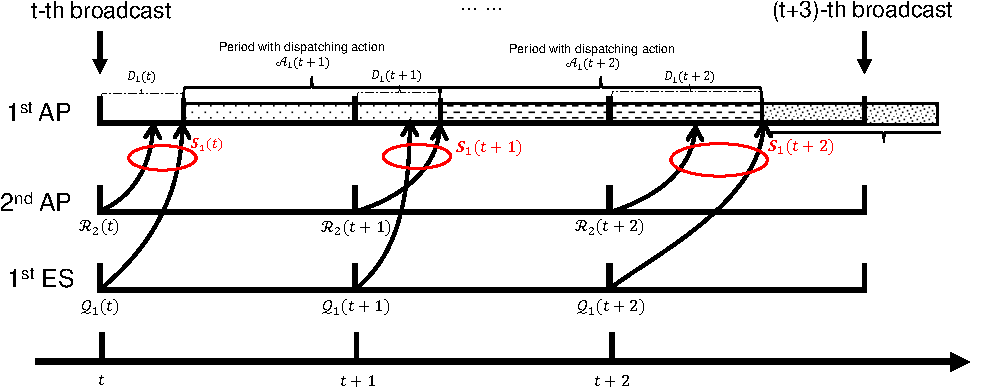
\includegraphics[width=0.60\textwidth]{brd-timeline.pdf}
%     \caption{The timeline illustration of reception of OSI for the $1$-st AP where $2$-nd AP is in its \emph{conflict AP set} and $1$-st server is in its \emph{candidate server set}.}
%     \label{fig:brd_timeline}
% \end{figure*}

The $k$-th AP is able to collect its OSI $\Stat_{k}(t)$ at the $\mathcal{D}_{k}(t)$-th time slots of the $t$-th broadcast interval, where $\mathcal{D}_{k}(t)$ \comments{denotes the \brlatency~of the $k$-th AP at the $t$-th broadcast interval which is a random variable in the unit of timeslot}.
It is assumed that $\mathcal{D}_{k}(t)$ follows identical and independent distribution in different broadcast interval.
% We refer to $\mathcal{D}_{k}(t)$ as the \brlatency~of the $k$-th AP at the $t$-th broadcast interval.
% An example is given below to demonstrate how the \brlatency~affects the reception of OSI and the update of the dispatching strategy.

% \begin{example}
%     In Fig.\ref{fig:brd_timeline}, the $2$-nd AP and $1$-st server are in the \emph{conflict AP set} and \emph{candidate server set} of the $1$-st AP, respectively.
%     At the beginning of the $t$-th broadcast interval, the dispatching actions $\mathcal{A}_{1}(t)$ is adopted by the $1$-st AP.
%     After $\mathcal{D}_{1}(t)$ time slots, it updates the dispatching actions to $\mathcal{A}_{1}(t+1)$ based on the OSI $\Stat_{1}(t)$.
%     At the beginning of the $(t+1)$-th broadcast interval, it will firstly keep the previous actions, and then updates the actions $\mathcal{D}_{1}(t+1)$ time slots later based on $\Stat_{1}(t+1)$ which is denotes as $\mathcal{A}_{1}(t+2)$.
%     The signaling latency $\mathcal{D}_1(t)$ and $\mathcal{D}_1(t+1)$ can be different.
% \end{example}
